\begin{tikzpicture}[align=center]
    
    \matrix[inner sep=0mm, column sep=1em, row sep=0mm] (mtx) {
        \node[inner sep=0pt, anchor=center] (trace) {
\includegraphics[height=.12\textheight]{img/floppy.png}}; 
        & 
        & \node[inner sep=0pt, anchor=center] (lego0) {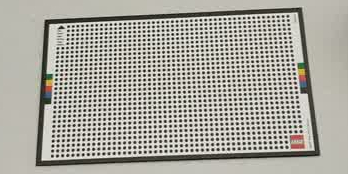
\includegraphics[height=.12\textheight]{img/lego/img0.jpeg}}; 
        & \node[inner sep=0pt, anchor=center] (lego1) {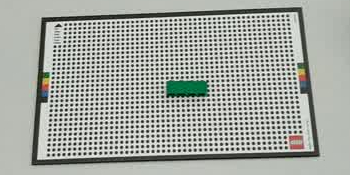
\includegraphics[height=.12\textheight]{img/lego/img1.jpeg}}; 
        & \node[inner sep=0pt, anchor=center] (lego2) {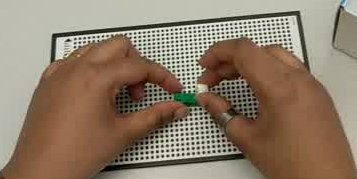
\includegraphics[height=.12\textheight]{img/lego/img2.jpeg}}; 
        & \node[inner sep=0pt, anchor=center] (lego3) {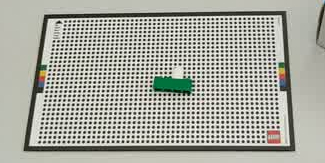
\includegraphics[height=.12\textheight]{img/lego/img3.jpeg}}; 
        \\
    };

    \node[fit=(lego0) (lego1) (lego2) (lego3), very thick, draw, rectangle] (fit) {};

    \begin{scope}[very thick, line cap=round]
        \draw (trace.east) -- (fit.north west);
        \draw (trace.east) -- (fit.south west);
    \end{scope}

\end{tikzpicture}